\section{Architecture and Design}
In this section we will discuss the specific solutions that we built in order to
achieve our goals, the motivations behind our design decisions, and the
technical challenges we overcame. Our project ended up being divided into a
series of independent components; Bee, our data agent; Hive, responsible for
storage and processing of data; Queen, our web front end; and finally, our iOS
application.

The key design decision was to build our system in a ‘Process Oriented’ manner.
This meant all components were broken down into small, scalable single task
components that did not maintain state. All state was stored in a central,
scalable database, and all communication was performed using a scalable
RabbitMQ\cite{rabbit} messaging exchange. Designing the system in this way meant
that we could leverage these technologies to provide a reliable, horizontally
scalable, and real time system.

\graphicspath{{./pics/}}
\begin{figure}[h!]
  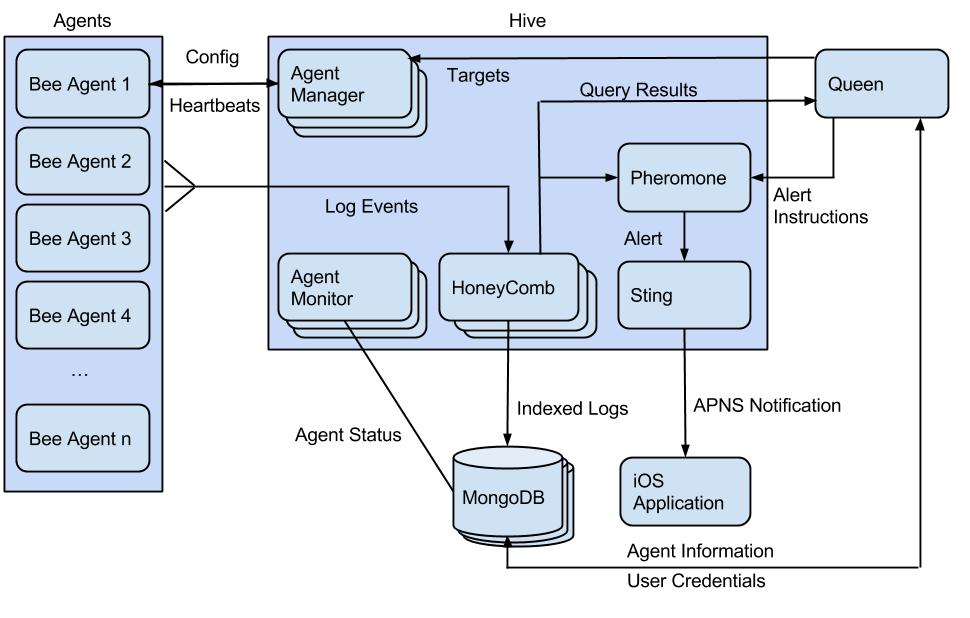
\includegraphics[width=8cm, keepaspectratio]{design.jpg}
  \caption{Design of Apiary Architecture}
\end{figure}


The reason for choosing RabbitMQ over other communication paradigms and
technologies, such as REST, is that it provides asynchronous message passing,
with worker queues and publish/subscribe models built in. Worker queues provide
automatic distribution of messages between Apiary components of the same type,
giving Apiary load balancing, and therefore configurationless scaling, for free.
The Publish subscribe model allows Apiary components to subscribe to real time
messages required for live events. It also maintains queues messages in the case
of congestion or component failure, ensuring no data is lost.

For the database we opted for MongoDB\cite{mongo}. We decided this was the best option
for the project because of the necessity to have very flexible data structures.
MongoDB stores collections of JSON objects instead of having rigid tables,
allowing for metadata and optional fields to be added dynamically to objects;
a feature that we specifically wanted for log entries. Due to the lack of
relations in MongoDB it is also known to scale very well, and because MongoDB
is JSON based like the rest of our stack, we would avoid data consistency
issues as no conversion would need to be performed between components.
